    % Chapter AddressFamily

\chapter{APNA Address Family} % Main chapter title

\label{address_family}
In this chapter we will discuss an approach to implement a new APNA address family for the SCION infrastructure. This chapter is structured as follows: Section \ref{addr:background} describes some background details about address family. \ref{addr:main_idea} covers the core idea behind this approach, followed by Section \ref{addr:tech} which discusses the technical difficulties and the modifications required in the current infrastructure. Section \ref{addr:data} presents an example in which two host communicate using the new address family. In the end we will discuss the drawback related to this approach \ref{addr:drawback}. 

\section{Background} \label{addr:background}
\subsection{What is an address family?}
\texttt{BSD} \texttt{socket()} API is the most fundamental API to create socket in any UNIX based operating systems. This BSD socket() API takes address family as a parameter (\texttt{address\_family}) which determines the address format of the structure to be used on socket APIs.

Address family protocols provide the network transportation of application data from one application to another (or from one process to another within the same system). The application specifies the network transport provider on the protocol parameter of the socket. For example the most popular address are following:
\begin{itemize}
    \item \textbf{AF\_INET address family} \\
    This address family provides inter-process communication between processes that run on the same system or on different systems.
    \item \textbf{AF\_INET6 address family} \\
    This address family provides support for the Internet Protocol version 6 (IPv6). AF\_INET6 address family uses a 128 bit (16 byte) address.
    \item \textbf{AF\_UNIX address family} \\
    This address family provides inter-process communication on the same system that uses the socket APIs. The address is actually a path name to an entry in the file system.
\end{itemize}

SCION's \texttt{SNET} library currently only support \texttt{AF\_INET} address family but there is a plan to support \texttt{AF\_INET6} address family soon. Apart from these traditional UNIX address families SCION supports two more address families \texttt{AF\_NONE} (represents None address type) and \texttt{AF\_SVC} (represents service address for SCION service) 

\section{Main Idea} \label{addr:main_idea}
Epiphany behind this approach is that we can introduce new address family \texttt{AF\_APNA} for APNA addresses. These addresses will represents the EphID used in the APNA communication session.

\subsection{Why do we need a new address family?}
In the approach presented in Chapter \ref{apna_overlay} there was one major drawback that it was wasting around 8-32 bytes depending upon whether endhost were using IPv4 or IPv6 address for communication. Conceptually speaking it was more of an hack rather than a well integrated solution inside SCION. 

Those bytes could be better utilized if we can introduce a new address family for APNA address. Instead of wasting space with random IPv4/IPv6 addresses use EphIDs as source and destination address. This would result in higher MTU for data packets as they don't have encapsulate EphIDs inside it and in the end would result in saving of lots of bytes which are better utilized by using EphIDs.

\subsection{Representation of APNA Address Family}
\paragraph{AF\_APNA address family}
This address family provides support for APNA protocol. AF\_APNA uses a 128 bit (16 bytes) Ephemeral IDs as address. Looking at the address size it looks very similar to IPv6 addresses but they have very different meaning. APNA address representation would be grouped as follows:
\begin{center}
deadcafe:baadf00ddeadbeef:40044b1d
\end{center}
First 4 bytes represents the initialization vector that was used to encrypt the host id. Next 8 bytes represents the encrypted host id. Last 4 bytes represents the MAC over first 12 bytes. Representation is not user friendly but it does not matter as users would never be using those addresses such as IPv4/IPv6 addresses as these are Ephemeral address and exists only for a short duration. Its representation is like that mainly for the debugging reason it makes it easy to identify what went wrong while generating EphIDs.

\section{Modifications required in the current infrastructure} \label{addr:tech}
There are various reason which contribute towards modifications in the current infrastructure. They summed up as follows

\begin{itemize}
    \item Border Routers needs modifications mainly due to two reasons: 1) Verifying packet authenticity before forwarding the packet to rest of the infrastructure 2) Change in the packet parsing logic because of new APNA address family.
    \item Dispatcher needs to be modified as well to understand this new APNA address family and decrypt EphID to find out the host IP address to forward the packet.
    \item Modification are required in the current SCION address library to introduce new APNA address family. Its much more involved than it sounds because it requires modification on Golang, Python and C implementation of SCION packet parsing.
    \item Modification are required in the library which constructs a SCION packet for the new APNA address family as well as for the new APNA header which resides inside SCION packet's payload.
    \item User-space library SNET which is used to establish communication inside SCION also needs to be modified as there are changes in the packet parsing with new APNA header.
\end{itemize}
\subsection{Border Router (BR)}
\paragraph{Source Border Router Modifications}
As we know from Section \ref{overlay:br_src} the major function that source border router needs to perform is packet authentication. And the changes required to verify packet authenticity are similar to mentioned in Section \ref{overlay:br_src}. Previously, it was obtaining source EphID from the payload but now instead of that its in the L4Header. Secondly end-to-end MAC is still present inside the payload where the APNA header is present. This MAC include source and destination EphID plus the data inside APNA packet. On a side note, this MAC could be distributed into two different types of MAC: 1) MAC over source and destination EphID and 2) MAC over real data inside APNA packet. But for the ease of implementation both of those were accumulated inside a single end-to-end MAC.

In order to verify packet authenticity need to register new hooks inside border router regarding \texttt{NeedsLocalProcessing} where it can extract the source EphID and obtain the relevant key from KMS to verify packet authenticity.

\paragraph{Destination Border Router Modifications}
The changes in the destination border are more less the same as mentioned in Section \ref{overlay:br_dst}. Its just the packet parsing logic is different and it does not replace destination EphID with decrypted IP address from it. That task is left for the dispatcher.  

\subsection{Intermediate Border Router}
All the intermediate BR needs to updated in this case as compared to previous approach. The reason behind that is packet parsing needs to adapt according to the new address family. This mainly due to reason how SCION packet is structured. Intermediate BR needs to read the path information to find out where to forward this packet. But apparently path information is present after the L4 header so in order to find the path information you need to find the correct offset inside the packet. The offset is determined by the looking at the address family inside the SCION Common Header. Hence all the intermediate BRs needs to be changed in order to make this approach work.

\subsection{Dispatcher}
Unlike the previous approach where BR was doing everything on behalf dispatcher with respect to handling EphID but for this approach solution is bit more complicated. The rationale behind that is in order to adopt a solution similar to previous approach would require re-writing of SCION packet but in theory BR do not modify packets. The intention would be to rewrite packet with IPv4/IPv6 as address family and replace those Ephemeral IDs to make it work. Since it required packet re-write we discarded this approach.

So we want dispatcher to understand this new address family. As far as decryption of EphID goes its easy just need to implement cryptographic primitive related to \texttt{AES-128} but inorder to obtain the IP address from HID is not trival. Since this operation would require contacting IMS but the dispatcher is written in C which makes things challenging. In order to communicate with IMS \texttt{CapnProto} specification needs to be compiled for C header files and this a lot of work to do.

There is a easy way out since every host needs to register with dispatcher in the SCION network initialization phase. So during that time we can hash the IP address of the host to obtain HID and store it inside a map. In order to obtain HID from IP address we need to implement cryptographic primitives related to Siphash and share the same key which IMS uses for generating the HID.

\subsection{SCION-APNA Packet Structure}
\begin{figure}[th!!]
\centering
\noindent
\makebox[\textwidth]{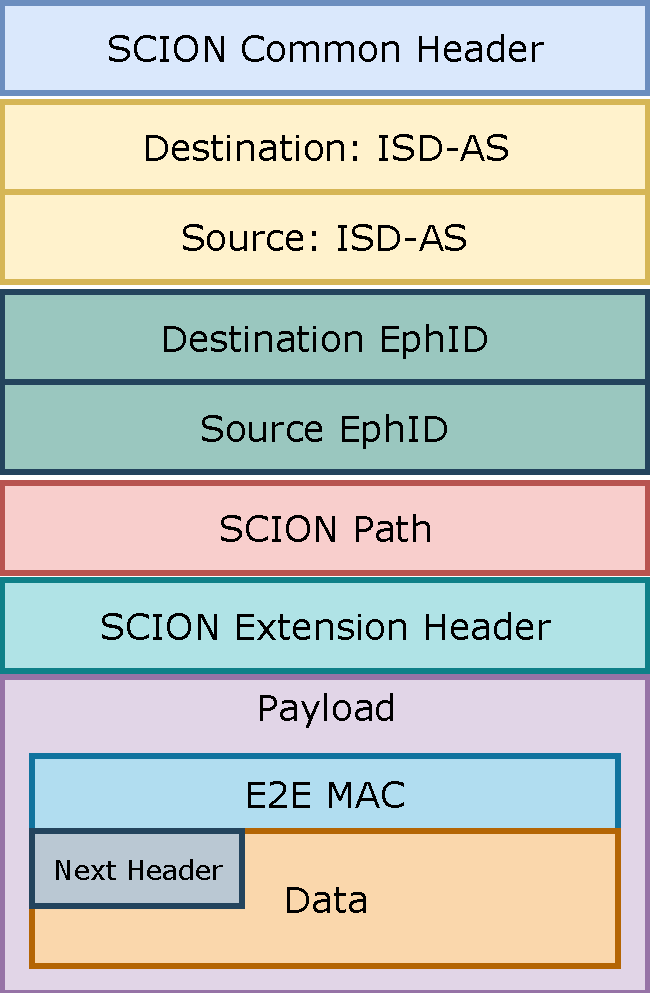
\includegraphics[scale=0.6]{Figures/apna_af.pdf}}
\decoRule
\caption[APNA packet structure using its own address family]{APNA Packet structure  using its own address family}
\label{fig:apna_scion_addr}
\end{figure}
Figure  \ref{fig:apna_scion_addr} exemplify a modified SCION packet which replaces IP address with Ephemeral IDs and payload gets extended with MAC and data.

\subsection{SCION Packet Parsing}

\paragraph{Golang}
\texttt{HostAddrType} enum needs to be extended with new \texttt{HostTypeAPNA} (4 is the numerical value) inside \texttt{go/lib/addr/host.go}. Since its a \texttt{HostAddrType} it needs to implement the other function in order to comply to the interface, which includes \texttt{Length}, \texttt{String} etc. 

\paragraph{Python}
\texttt{HostAddrBase} map needs to be extended to support this new APNA address family. The changes are contained within one single file \texttt{python/lib/packet/host\_addr.py} and are similar to Golang.

\paragraph{C}
The changes required on the C side are contained within \texttt{c/lib/scion} subsystem apart from the changes which are required from dispatcher. A new macro \texttt{ADDR\_APNA\_TYPE} needs to be introduced with its associated length macro inside \texttt{c/lib/scion/address.h}

\subsection{SNET}
First of all \texttt{SNET} requires a similar change as the previous approach i.e., a new network string parameter "apna". Rest of the changes regarding APNA handshake and session management is similar to one mentioned in Section \ref{overlay:snet}

\section{Data Communication} \label{addr:data}

\begin{figure}[th!!]
\centering
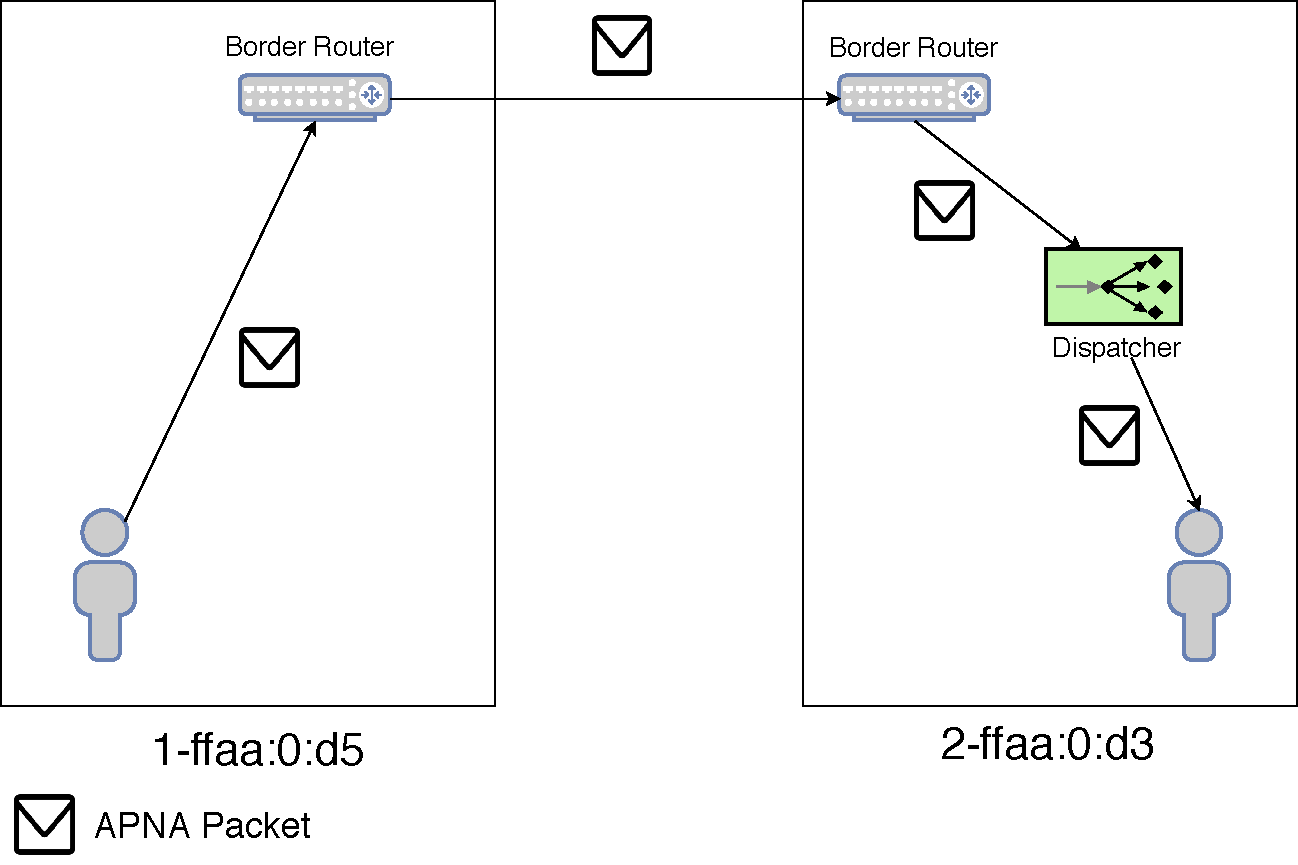
\includegraphics[scale=0.5]{Figures/address_family_comm.pdf}
\decoRule
\caption[APNA Service Incoming Packet]{Communication overview using APNA address family}
\label{fig:apna_address_comm}
\end{figure}
Fig \ref{fig:apna_address_comm} represents a scenario in which Host A in ISD 1 and AS \texttt{ffaa:0::d5} wants to communicate with another Host B in ISD 2 and AS \texttt{ffaa:0::d3}. 
It only presents a very abstract idea as most of details are same as previous approach.
There are four major parts

\subsection{Part One: Sending packet to first hop BR }
This part involves setting up the SCION networking context first similar to the previous approach and query the path server using SCIOND to obtain a list of available to Host B. From the list Host A can choose any path that he likes depending upon his requirements/constraints. After selecting the path, Host A can perform DNS query resolution for Host B and obtain its receive-only EphID registered with DNS Service. After that using the SNET API host can construct the SCION-APNA packet and send it to the border router interface mentioned in path-set returned by the Path Server.

\subsection{Part Two: Routing packet to last hop BR}
Once the packet reaches first hop border router it will verify the packet authenticity and if that's successful it will forward the packet to the next hop border router looking at the path information header inside the SCION packet. All information that is needed to forward the packet is present inside the packet until the packet reaches the last hop border router.

\subsection{Part Three: Forwarding packet from last hop BR to Dispatcher}
For this part last hop border router needs to decrypt destination EphID to obtain the IP address associated with the dispatcher. In order to do so its better than previous approach because it does not need to completely parse the packet to obtain the destination EphID. And with the help of IMS it can easily decrypt destination EphID. After that it can easily forward the packet using the UDP overlay.

\subsection{Part Four: Forwarding packet to endhost from Dispatcher}
One packet has reached the dispatcher it needs to parse the packet to obtain the destination EphID and using the AES key it can decrypt EphID to obtain HID. Since it has already created a mapping between HID and IP address during the initialization phase it can use that mapping to obtain IP address from HID instead of contacting IMS for it. After that packet is forwarded using a UNIX domain socket to Host B.

% \subsection{Algorithm to obtain IP address from EphID} \label{algo:addr_fam_comm}
% \begin{algorithmic}
%  \STATE $P \leftarrow $ Parse the SCION Packet
%  \STATE $DstEphID  \leftarrow P.L4Header.DstEphID $ 
% \end{algorithmic}
  
% \begin{algorithmic}
%  \IF{$DstEphID$ is not nil}
%  \STATE $HID \leftarrow Decrypt(DstEphID)$
%  \IF{$HID$ is not nil}
%  \STATE $IP \leftarrow GetIPFromHID(HID)$
%  \ELSE
%  \STATE Drop the packet and abort; 
%  \ENDIF
%  \ELSE
%  \STATE Drop the packet and abort;
%  \ENDIF
% \end{algorithmic}

\section{Drawbacks} \label{addr:drawback}
The main drawback behind this approach is that it requires changing all the intermediate border routers to deploy this approach on any existing SCION deployment. Changing all the intermediate border routers is not really solution for someone who wants to experiment with the prototype implementation. So is there no way out of this problem? I think there is a way using SCION service infrastructure and offload some functionality of the border routers to a new SCION service. We will discuss more about this approach in the next Chapter.